\section{Signal Start Detection}
\label{sec:04_signalStartDetection}

Previously, the importance of the signal start was underlined
due to the fact that the direction detection methods is
executed on smaller frames.
To demonstrate this for the phase method, the frame to investigate is
shifted with time \cref{subsec:04_frameNumber}.
Results in show that in fact, the accuracy decreases with sliding frame.
According to the outcome of \cref{subsec:04_psnr}, also for the \ac{GCC}
method performs best with frames near to the signal start.

There are some reasons why other methods were tested to find the signal start.
One is that the existent whistle detection algorithm of \cref{subsec:03_whistleDetection}
is computationally intensive.
However, for high accuracy either the number of samples in a frame have to be
small or the window must be shifted with small steps which both implicit
a high number of executions.
In addition, for small frames the whistle detection is causes false positives
as \label{subsec:04_whistleDetection} shows.
Lastly, the detection is restricted to whistle sounds only.

Hereinafter, the characteristics of the methods are pointed out by
analyzing the error between algorithmically determined start index
and manually set start index.


\subsection{ZCR}
\label{subsec:04_zcr}

Performance of the \ac{ZCR} whistle start method is evaluated by taking the eleven
measurements on all five robots of \cref{subsec:04_labMeasurements} into account.
In many cases, the method provides good results.
The frame size is set to 256 samples and both, number of noise and signal frames
are set to 10.
For example, the eleven measurements done with robot 26 at the center point
are precise with only a \ac{RMSE} of 54,23 samples.
In 17 cases of all four channels of the 55 measurements (7\si{\percent}),
the method missed the start index with a significant error larger than 256 samples.

However, there are cases where the algorithm fails due to incorrect assumptions.
One assumption is that the signal is represented at the end of the buffered
samples.
Some measurements prove, that this is not always the case as in \cref{fig:04_zcrFail}.
Here, the data of the front right channel of robot 21 with the whistle source
at position 5 of \cref{subsec:04_labMeasurements}
shows that the signal is not represented at the last part of the buffer.
Hence, if the start index is determined by the first index lower than
the threshold by looking at the \ac{ZCR} backwards.
In this measurement, the \ac{RMSE} of the remaining three channels is
51,45 samples.
In most cases where the algorithm fails, only one channel of four
is erroneous.
Because the final start index on one robot is set equal for all channel,
the failure can be compensated with a smart voting procedure.
% -------------------------------------------------------------
\begin{figure}[ht]
	\centering
		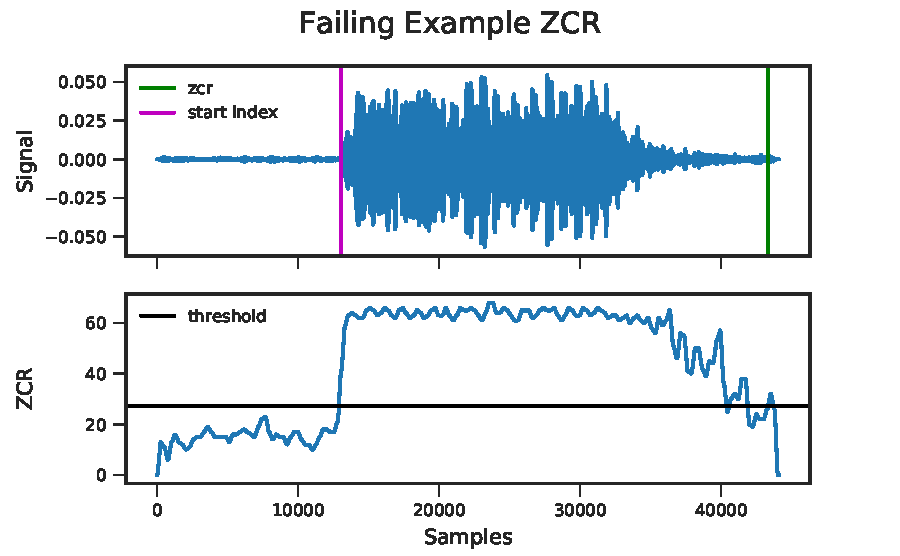
\includegraphics[]{figures/evaluation/zcr_fail}
    \caption{Channel 3 data from measurement 5 of \cref{subsec:04_labMeasurements}
             for robot number 21. A failing example for the start detection by \ac{ZCR}
             is shown.}
	\label{fig:04_zcrFail}
\end{figure}
% -------------------------------------------------------------

Another option exists by changing the process of finding the
threshold excess onwards.
In this case, the threshold is raised with a factor of 1,25.
Results by this were poorer than the initially implemented manner
with 15\si{\percent} channel results with larger error than 256 samples.
By adding the constraint that following frames also need to exceed the
threshold, result can be improved slightly but implies higher
computational effort.

Worth mentioning is the poor output of the \ac{ZCR} method with
signal that was cleaned with spectral subtraction previously.
This surprising outcome is convenient for the overall task,
because the start index result can be embed into the spectral
subtraction, providing information for separating the noise
and signal part.

\subsection{Entropy}
\label{subsec:04_entropy}

The entropy quantifies the amount of chaos in a signal frame.
Especially for signals to localize with unknown characteristics,
this method can be useful if results are promising.
For all measurements on all robots of \cref{subsec:04_labMeasurements}
the results are poorer than the \ac{ZCR} method in \cref{subsec:04_zcr}
with around 20\si{\percent} failure rate.
Best results are achieved with a frame size of 512 samples and a difference
step of 800 samples. \change[]{Explain what steps are? Maybe in implementation?}
However, for records with fading whistle data the entropy method
generates more reliable results.
Taking such a measurement as an example, \cref{fig:04_entropyGood}
shows how the algorithm detects the signal start correctly even though
the whistle sound ended around 38000 samples.
This data corresponds to the one in \cref{fig:04_zcrFail} and demonstrates
the difference to the \ac{ZCR} method exemplary.
For this measurement, errors of the start indexes for all four channels
are smaller than 40 samples.
In comparison, three channels fail with the \ac{ZCR} method in this case.
% -------------------------------------------------------------
\begin{figure}[ht]
	\centering
		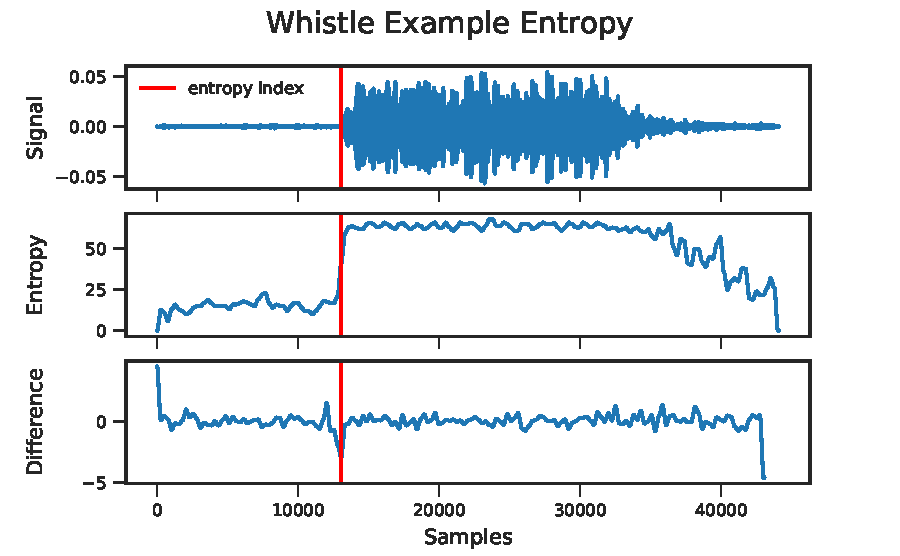
\includegraphics[]{figures/evaluation/entropy_good}
    \caption{}
	\label{fig:04_entropyGood}
\end{figure}
% -------------------------------------------------------------

% But as the entropy should be larger for noisy environment
% performance in other surrounding of measurement at robocup is looked at.
% Entropy would be best for undefined signal -> distinguish between
% signal and noise without information

\subsection{Whistle Detection}
\label{subsec:04_wd}

For the purpose of detection the start of a whistle signal, the whistle
detection can be utilized.
9\si{\percent} 23\si{\percent} with np.argmax(), looking at the next 300
values and with a step size of 50 the result is 15\si{\percent} and 36\si{\percent}
and with step size 1, it is 13\si{\percent} and 33\si{\percent}.
This is computationally very costy and the reward is small.

\subsection{Start Detection Conclusion}
\label{subsec:04_startDetectionConclusion}

If the start of a whistle sound is wanted and computational effort is
neglected, the evaluation shows that the start detection with the
existing whistle detection algorithm performs best.
that a rough start detection by the exiting whistle detection
with a large frame size followed by a \ac{ZCR} detection with small
window size.
This is a good trade-off with regard to the computational effort.
\change[inline]{change for more noisy signals? -> then maybe entropy?}
% - entropy for large scale start detection\\
% - zcr and energy for smaller scale (because high precision needed)\\